\newcommand{\bm}[1]{\textit{#1}}
%test
% Copyright
%\setcopyright{none}
%\setcopyright{acmcopyright}
%\setcopyright{acmlicensed}
%\setcopyright{rightsretained}
%\setcopyright{usgov}
%\setcopyright{usgovmixed}
%\setcopyright{cagov}
%\setcopyright{cagovmixed}
% DOI
\setlength{\textfloatsep}{0.1cm}

\chapter{Dynamic runtime adaptation for efficient execution}\label{chp:cases}


Chip Multicore Processors (CMP) are now ubiquitous in embedded computing as single threaded performance improvements have slowed.
CMPs have to be carefully designed, balancing the size of each core with the total number of cores on the chip.
Larger cores are typically good at exploiting instruction level parallelism (ILP) but might potentially be very power hungry.
Smaller cores on the other hand require less power but offer limited performance, forcing software developers to parallelize their code with multiple threads, which is a tedious process.
As the size and the number of cores is fixed at design time, choosing the right balance is difficult~\cite{DubachExpl2012, TomuskHet2015}.

Asymmetric Chip Multicore Processors (ACMP) have been proposed~\cite{MittalSurv2016} to overcome this issue.
These processors feature either different sized cores~\cite{JibajaPPerf2016} or different Instruction Set Architectures~\cite{VenkatISADiv2014} to efficiently tackle a multitude of different workloads.
Dynamic Multicore Processors (DMP) push this further by introducing Core Fusion~\cite{ipek2007CoreFusion}.
Similar to ACMPs, Core Fusion allows the chip to have different sized cores, but this can be changed at runtime.
In a DMP, cores can be fused dynamically to create larger cores similar to a superscalar processor.
Any number of cores can potentially be combined together whenever a workload exhibits a large amount of ILP.
When a program exhibits low ILP, the DMP can decouple fused cores to conserve energy.

While a large number of DMPs have been proposed in the literature~\cite{ipek2007CoreFusion,pricopi2012bahurupi,kim2007tflex,Watanabe2010Widget}, these efforts focus on the hardware and microarchitectural design.
They evaluate the hardware using a fixed number of fused cores or provide an oracle for dynamic fusion.
There exists little~\cite{micolet2016dmpstream} to no literature on predicting core fusion from a software perspective.
To the best of our knowledge, there has been no study on dynamically changing the number of cores fused to better match the phases of a workload in a homogeneous DMP compared to ahead of time fusion.

We start with an explanation of the theoretical limitations of core fusion and what we can expect in terms of performance.
We then discuss how classical loop optimizations such as unrolling can have a large impact on performance when fusing cores.
Using the San Diego Vision Benchmark Suite~\cite{sdvbs} (SD-VBS) as a use case, we show that programs exhibit various phases with different amounts of ILP.
We then perform a limit study on the potential for decreasing energy consumption while maintaining performance when adapting the number of cores for each program phase.
Our results show that using dynamic core fusion can save up to 42\% on average while maintaining the same level of performance as a fixed number of cores.
We also show how latency introduced by reconfiguring the system can influence the impact of core fusion.
Finally, we build a simple online model using linear regression that predicts the optimal number of cores per phase for reducing energy consumption while maintaining performance.
This practical model leads to an average of 37\% saving in energy with no performance loss.

To summarize, our contributions are:

\begin{itemize}
\item We analyze the limits of core fusion using an analytical model.
\item We study the loop optimizations required to ensure efficient use of core fusion.
\item We offer an in-depth comparison of static and dynamic core fusion schemes on the San Diego Vision Benchmark Suite.
\item We show that core fusion has the potential to offer a large reduction in energy savings.
\item We show how a simple linear-regression based model can predict the number of cores to fuse for different program phases.
\end{itemize}



%\section{Dynamic Multicore Processor}\label{sect:background}
%\paragraph{Dynamic Multicore Processor} DMPs contain hardware which can be modified post fabrication.
Mitall's survey ~\cite{MittalSurv2016} defines three types of modifiable resources: the core count~\cite{ipek2007CoreFusion}, number of resources that each core has~\cite{Homayoun3DPooling2012} and micro-architectural features~\cite{fallinhetblock2014,BauerRSE08,tavanaElastic}.
In our paper we focus on DMPs that modify the core count.

\paragraph{EDGE ISA} We assume a DMP similar to TFlex~\cite{kim2007tflex} using an Explicit Data Graph Execution~\cite{burger04edge} (EDGE) instruction set architecture (ISA).
EDGE ISAs encode dependencies between instructions at the ISA level.
Code is organised as blocks of instructions where all instruction communication is local to the block~\cite{smith2006edge}.
Each block has a single entry point but may have multiple exits.
This enables the architecture to dispatch blocks speculatively, with low overhead~\cite{putnam2010e2,kim2007tflex}, therefore, increasing exploitation of ILP.

 \begin{figure*}[t]
 \center
 \includegraphics[width=1\textwidth]{cases-paper/graphics/background/proc_test.pdf}
\vspace*{-5mm}
 \caption{Core Fusion Mechanisms for our EDGE-based architecture.}\label{fig:dmp}
\vspace{-5mm}
 \end{figure*}
\paragraph{Core Fusion} 
Core Fusion is achieved by fusing a set of \textit{physical} cores to create larger \textit{logical} cores.
This does not modify the physical structure of the chip, instead it provides a unified view of a group of physical cores to the software.
For example, fusing two cores generates a logical core with twice the amount of execution units, register files and L1 cache.
Fusion is a dynamic modification and may occur during the execution of a program to better fit the workload.
Unlike traditional CMPs, fused cores will operate on the same thread and attempt to extract Instruction Level Parallelism (ILP) rather than Thread Level Parallelism (TLP)~\cite{micolet2016dmpstream,pricopi2012bahurupi}.
Figure~\ref{fig:dmp} shows the different stages and mechanisms of core fusion for a four core system.
When creating a new core fusion a master core informs all other cores about the fusion and sends the predicted next block address to the next available fused core.
When a core mis-predicts a branch in a fusion, it informs the other cores which flush any younger blocks.
When un-fusing, the master core informs the other cores, which then commit or flush their blocks and power down while the master core continues to fetch and execute blocks from the thread.
The extra hardware required to support dynamic reconfiguration is very minimal~\cite{kim2007tflex} since most of the machinery already in place can be reused such as the cache coherence protocol when fusing and un-fusing the cores.
We discuss this in further detail in Section~\ref{sec:setup}.


\section{Motivation}\label{sec:motivation}
This section motivates the use of dynamic core fusion and its impact on performance and energy.
It also shows that loop optimizations have a significant performance impact when fusing cores.

\subsection{Dynamic Core Fusion}
\begin{figure}[t]
    \centering
    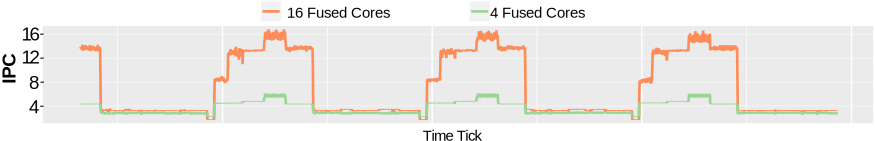
\includegraphics[width=\textwidth]{cases-paper/graphics/motivation/disp_opt_4_16_3.pdf}
    \caption{IPC of a typical benchmark (Disparity from SD-VBS) when executing on a fused 4 or 16 core processor.} 
    \label{fig:disp_ex}
	\vspace{1em}
\end{figure}
%\begin{figure}[t]
%    \centering
%    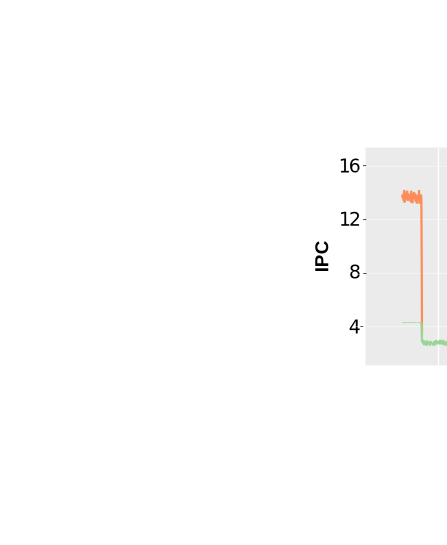
\includegraphics[width=\textwidth]{cases-paper/graphics/motivation/motiv3merge.pdf}
%    \caption{Example of ideal switching between 4 and 16 cores on a DMP for the Disparity benchmark.} 
%    \label{fig:ideal_switch}
%\vspace{2em}
%\end{figure}

Previous work in core fusion focuses on delivering performance improvements~\cite{ipek2007CoreFusion,kim2007tflex} and demonstrates how to predict static core fusion~\cite{micolet2016dmpstream}.
A static fusion fuses cores into a single logical core (LC) and executes a thread on this new core.
As evident from this prior work, fusion improves the performance of the program by maximizing speed.
However, as will be shown, static core compositions may not be the perfect match for all situations.

Figure~\ref{fig:disp_ex} plots the Instruction Per Cycle (IPC) performance variation over the execution of the \bm{Disparity} Benchmark from the San-Diego Vision Benchmark Suite (SD-VBS)~\cite{sdvbs} on core compositions of sizes 4 and 16 respectively.
IPC is a natural method of evaluating the performance of a core-composition as increasing the size of the composition should lead to a higher amount of instructions executing per cycle.
On 4 cores, the performance oscillates between an IPC of 2 and 6 depending on the phase while on 16 cores the IPC can be as high as 16.

In this Figure, the x-axis Tick represents a certain number of blocks that have been committed rather than being a measure of time in cycles.
This is why the high IPC phases for both core-compositions appear to last the same length of time even though the 16 core-composition executes the blocks faster.
In EDGE, a block is committed when it is no longer a speculative block and its memory and register operations have been committed back to memory or the register files.
The reason why number of blocks committed is used as a measurement of time is due to the fact that the number of blocks necessary to execute a program are independent of the size of a core-composition.

As can be seen in Figure~\ref{fig:disp_ex}, both the 4 and 16 core-compositions share the same IPC when it comes to the low IPC phase.
In a situation where the objective of the programmer is to maximise speed, without dynamic reconfiguration of the DMP, a static 16 core-composition will have to be used.
%Get actual energy estimations ot make this more clear
If the static 16 core composition is used, the DMP consumes 4 times as much energy to execute the low IPC phases compared to the 4 core-composition.
Thus, the static 16 core composition is considered energy inefficient during half the execution of the program.

On the other hand, if the DMP is reconfigured at runtime, the core-composition can switch to 4 cores when in the low-IPC phase to save on energy and switch to the 16 core composition when in the high IPC phase to maximise speedup.
In this situation, runtime reconfiguration allows to maximise speed whilst being energy efficient; a goal that cannot be achieved via static ahead of time configurations.

%Maybe, just maybe, add a graph showing how the size of the blocks change (need data on this).
\subsection{Code Optimizations}

When cores are fused they execute blocks of instructions in parallel on each physical core in the core composition, also known as a logical core (LC).
Having multiple cores in a composition can increase the amount of block level parallelism (BLP) that can be extracted out of a program.
A high amount of BLP leads to high IPC as each core in the LC executes their block in parallel.
As IPC is a more commonly used method of measuring performance, it is used throughout this chapter.
In order to obtain the best performance from an application, large blocks must be generated as this leads to a higher IPC on the LC as described in Chapter~\ref{chp:streamit}.
To summarise the reasons, which are also discussed in further details in Section~\ref{sec:lim_study}, larger blocks reduce the latency caused by having to fetch blocks for all the physical cores in the LC, thus improving performance.

Thus, optimisations that maximise block size will positively affect the performance of compositions.
This includes optimisations such as aggressive loop unrolling, inlining and replacing conditional statements with either software predication or architecture-level predication.
These optimizations are well known and do not require any structural modifications of the program.

\begin{figure}[t]
    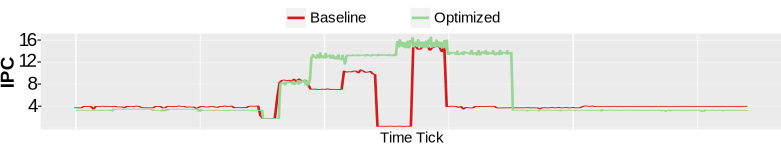
\includegraphics[width=\textwidth]{cases-paper/graphics/motivation/code_opt_3.pdf}
    \caption{Impact of loop transformations on fused cores for the Disparity benchmark.} 
    \label{fig:compmotiv}
\vspace{1em}
\end{figure}

Figure~\ref{fig:compmotiv} illustrates the impact of applying loop transformations on the \bm{Disparity} benchmark compared to a standard compiler not specifically tuned for the EDGE architecture.
The Figure shows the IPC performance of a 16 core composition with and without optimisations.
As can be seen, the impact of these transformations can be large, leading to an 12x improvement on IPC.
Figure~\ref{fig:compmotiv} shows that the optimisations allow the core-composition to sustain a high IPC phase longer than without the optimisations.
However, it also demonstrates that not all of the code in a program can be optimised, as the low-IPC phases do not change.
More details about the loop transformations are given in section~\ref{sec:opt} but this example illustrates the need for careful tuning of the compiler to achieve high performance on such an architecture.

%Find some citation for this
\subsection{Automating runtime reconfiguration}

Figure~\ref{fig:disp_ex} motivates the use of runtime reconfiguration to ensure that DMP can improve the performance of single threaded applications efficiently by minimising energy consumption.
Figure~\ref{fig:compmotiv} shows how modifying loops affects the performance in terms of IPC for a core-composition.
Using an API, a programmer could inform the hardware when to reconfigure by using specific functions or pragmas similar to OpenMP or OpenCL.
Whilst this may be considered a viable approach to applying runtime reconfiguration, automating the decision process is a better option.

Automating the process of reconfiguring the processor enables two advantages compared to manually determining when to reconfigure the processor.
The first advantage is that it removes the responsibility from the programmer: an automated runtime reconfiguration system can detect phases and adapt to them accordingly, using information gathered from previous traces.
Second, if ever the program is modified, this may require new profiling information to be generated to ensure that manual reconfiguration calls are correct.
If the reconfiguration is automated, then it can adapt automatically to any changes made to the source code.

\subsection{Summary}
This section has shown that programs exhibit phases with various amount of ILP available.
A dynamic multicore processor can take advantage of this property to fuse a large number of cores for the high-ILP phases and fuse a smaller number of cores when ILP drops to conserve energy.
The section also illustrated the importance of fine-tuned code transformations to achieve sustained performance and increase the potential for fusing cores.
The next section will study in more details the expected impact of fusion using an analytical model.



\section{A Study of Core Composition}\label{sec:lim_study}
This section studies how block size and branch prediction limit the performance of core composition.
This enables a better understanding of what leads to good performance and how to determine regions of code that benefit from core composition.

\subsection{Branch Prediction}


As discussed in Chapter~\ref{chp:Background}, an EDGE based DMP accelerates a single thread by executing blocks of instructions from the same thread speculatively across several fused cores. 
In a core composition, the fetching scheme dictates that a core must fetch blocks until its instruction window is either full or cannot accomodate the newest block.
Once this requirement is met, the following block is sent to the next core in the composition.
If a core mispeculates a block, this can cause the entire composition to be flushed.
Thus core composition puts a strain on the branch predictor since efficiently using the cores depends on the prediction accuracy.

Depending on the sizes of the blocks and the number of cores in the composition, the branch predictor has to meet a different accuracy requirement to ensure all cores are being used efficiently.
In this case, efficiency is defined by cores in a composition successfully fetching correctly predicted blocks.
Given a core-composition of size \textit{CompSize}, the minimum branch prediction accuracy required to ensure efficient use of the composition can be determined using Formula~\ref{form:minpred} where \textit{BlocksInFlight} can be calculated using the equation~\ref{form:blocks}.

\begin{equation}\label{form:blocks}
BlocksInFlight(AverageBlockSize) = \begin{cases}
4, &\text{if } AverageBlockSize \le 32 \\
3, &\text{if } 32 < AverageBlockSize \le 64 \\
2, &\text{if } 64 < AverageBlockSize \le 96\\
1, &\text{if } 96 < AverageBlockSize\\
\end{cases}
\end{equation}

\begin{equation}\label{form:minpred}
PredAcc(ABS,CompSize)= \frac{BlocksInFlight(ABS) \times CompSize- 1}{BlocksInFlight(ABS) \times CompSize}
\vspace{1em}
\end{equation}

\textit{BlocksInFlight} represents the number of blocks that can execute on a single core in parallel.
There can be multiple blocks on a single core as the instruction window has four lanes per core.
In this thesis, the instruction window is 128 instructions wide, thus each lane can support a block of up to 32 instructions.
In Equation~\ref{form:minpred}, the -1 is due to the fact that when a program is executing the first block does not depend on a branch prediction, thus at any point during the execution of a program, there is a non-speculative block that does not need to predicted.

Figure~\ref{fig:req_pred} shows the expected prediction accuracy required to fully utilize a core composition given the average block size in flight.
In this figure, \textit{NumOfBlocksPerCore} is equal to four and \textit{MaxBlockSize} is 32.
Adding extra physical cores to a LC requires an increasingly accurate branch predictor, especially when the size of a block is under 50 instructions.
This provides two insights; first of all large LCs will need to run on code sections with less control flow as they are more sensitive to branch misspredictions.
Second of all, branch prediction can be a simple method of evaluating the current effectiveness of a LC.
Given a certain number of cores, if the prediction accuracy is under the limits presented in Figure~\ref{fig:req_pred} it can be easily determine that the LC is sub-optimal.

\begin{figure}[t]
    \centering
    \includegraphics[width=\textwidth]{cases-paper/graphics/limit_study/prediction_req.pdf}
    \caption{Required prediction accuracy for a logical core size to be efficient given an average block size.}
    \label{fig:req_pred}
	\vspace{1em}
\end{figure}

\subsection{Synchronization Cost}

For a program to execute correctly, the cores in a logical core (LC) must communicate when they have finished executing a block.
This ensures that the cores fetch blocks from the correct control paths and update memory and registers consistently.
A core may have to wait for other cores to commit before fetching a new block. 
The worst-case estimate of this stall is defined as the \textbf{Synchronization Cost}.

Blocks commit in a sequential fashion with the non-speculative block committing first and the most recent speculative block committing last.
If a core's instruction window is full then it must commit a block before it fetches a new one.
The Synchronization Cost, in cycles, is defined in equation~\ref{form:synccost} and is measured by averaging the overall number of cycles each fused core waits until it can continue to fetch and execute new blocks.
\textit{AvBlocksInFlight} represents the average number of blocks in flight on a single core in the LC.
This is a worst-case estimate as block sizes will fluctuate during the execution of a program.

\begin{equation}\label{form:synccost}
SyncCos(ABS,CompSize) = \frac{\sum_{CoreNumber=0}^{CompSize-1}\left(BlocksInFlight(ABS)\right) \times CoreNumber }{CompSize}
\end{equation}


Figure~\ref{fig:sync_cost} shows how many cycles the Synchronization Cost will be for a given LC and average block size.
The larger the block size the lower the Synchronization Cost is since cores fetch fewer blocks and wait less for other fused cores to finish committing.
Large LCs executing small blocks have a high Synchronization Cost. 
This indicates that large LCs should be avoided when dealing with smaller blocks as the Synchronization Cost outweighs the code execution.

\begin{figure}[t]
    \centering
    \includegraphics[width=\textwidth]{cases-paper/graphics/limit_study/sync_cost.pdf}

    \caption{Synchronization Cost in cycles for a given number of cores in a composition and an average block size.} %Each core has 4 lanes and each lane can fetch a block of up to 32 instructions. Lower is better.}
    \label{fig:sync_cost}
	\vspace{1em}
\end{figure}

\begin{figure}[t]
    \centering
    \includegraphics[width=0.8\textwidth]{cases-paper/graphics/limit_study/summary.pdf}
    \caption{IPC estimate given a logical processor size, average branch prediction and average block size for a dual-issue core. A higher IPC means better performance.}
    \label{fig:lm_summ}
\vspace{5mm}
\end{figure}


\begin{align}\label{form:wcetMath}
IPC(ASB,CS,BPredAcc) &= \bigg(\frac{ABS}{SyncCost(ASB,CS) + {\frac{ASB}{2}}}\bigg) \times BPredAcc \times CS
\end{align}


\paragraph{Summary}

This section estimates the worst-case IPC for a logical processor using Average Block Size, Average Branch Prediction, and Synchonization Cost.
Figure~\ref{fig:lm_summ} presented a worst-case estimate of IPC performance assuming each core can sustain an IPC of 2.
The figure is generated by assuming that cores can execute 2 instructions per block, and using the two previous formulas with different block sizes, accuracies and core composition sizes to generate estimated IPC values.
The formula used is defined in equation~\ref{form:wcetMath} where \textit{ASB} represents the average size of a block, \textit{CS} is the size of the composition and \textit{BPredAcc} is branch prediction accuracy that ranges from 0 to 1.
From what was previously explained, Figure~\ref{fig:lm_summ} shows us that to obtain optimal performance requires a high branch prediction accuracy and large blocks.
It shows that larger logical processors can easily under-perform; for example it can be seen that 16 fused cores often have IPCs under 15, meaning that each core has an IPC under~1.



\section{Methodology}\label{sec:setup}
The previous section studied the performance potential for core fusion using an analytical model.
We now present the experimental setup used for the remaining parts of the paper where we conduct a thorough evaluation of core fusion with a cycle-level simulator.

\subsection{Benchmarks}

For this paper we study the performance of our Dynamic Multicore Processor (DMP) on a set of Vision Benchmarks designed for hardware and compiler research~\cite{sdvbs}.
The San Diego Vision Benchmark suite (SD-VBS) is composed of nine single-threaded C benchmarks ranging from image analysis to motion tracking.
These benchmarks represent state-of-the-art applications in image and vision recognition which are prevalent in embedded systems.

Vision applications typically have regular and simple control flow which enables the formation of large blocks of instructions.
Our processor relies on the ability to form large blocks to exploit ILP which makes these applications particularly well suited.
As the results will show, the phase length has minimal impact on energy savings when the reconfiguration overhead is low.

\subsection{Architecture and Simulator}

We use a cycle-level simulator of an EDGE-based Dynamic Multicore Processor~\cite{e2} whose core pipeline is verified against an RTL implementation within 5\%. 
This validation is done by running workloads on RTL and comparing the traces cycle-by-cycle with the software simulator.
The architecture and core fusion mechanics are similar to the work described in~\cite{kim2007tflex,putnam2010e2}.
We configure the simulator to model a 16 core multiprocessor, with 32 KB private L1 caches, and allow each core to fetch up to 4 blocks of instructions, 
and issue up to 2 instructions per block for a maximum of 64 blocks in flight.


\subsection{Fusing Cores} \label{sec:coresufion}

In this processor, the micro-architecture is distributed: register files, Load Store Queues (LSQs), L1 caches and ALUs all look like nodes on a network.
This means that when cores fuse together, this is similar to adding an extra node to the network.
When cores are fused, one of the cores will execute a non-speculative block from a single thread whilst all other cores execute speculative blocks that are predicted from the same thread.
For our study, we use a simple round robin policy to choose which core is going to execute the next speculative block.
When we start a new thread on a fused core the OS and runtime write the new core mapping to a system register.
The hardware then flushes these cores if they are not idle and sets the PC of the first block of that thread on one core in the logical processor and starts executing.

Fusing cores is therefore a lightweight process.
We estimate that switching the size of the logical-core (LC) results in a delay of 100 cycles on average.
The actual time varies based on the time it takes the cache coherence protocol to move the data around the memory system.
Section~\ref{sec:reconfoverhead} discusses in more details how latency affects energy efficiency and shows that dynamic core fusion is still highly beneficial even when considering overheads of 1,000 cycles.

\subsection{Compiler}
Each benchmark is compiled with the Microsoft C++ compiler for EDGE~\cite{e2}, with -O2 optimisations and using instruction predication for hyperblock formation~\cite{smith2006edge}.

\subsection{Measuring Performance and Power}

We run five simulations per benchmark, one for each LC size: 1, 2, 4, 8 and 16.
For each LC we record the IPC of the LC at an interval of 640 committed blocks.
We selected 640 committed blocks as it allows each core in a LC to execute enough blocks before taking the measurement.
This is due to the fact that the highest LC of 16 cores can execute up to 64 blocks at a time, thus recording performance after 640 blocks allows each core to have executed at least 10 blocks.
Using committed blocks as an interval allows us to easily compare each simulation as the total number of committed blocks does not change even if the LCs are different.

Due to the fact that we study an EDGE ISA~\cite{smith2006edge}, we cannot use McPAT to model power consumption as it differs from traditional CISC/RISC cores modeled in McPAT.
Instead we use a coarse grained power model where either a core is turned on or or it is off. 


\section{Code Optimizations}\label{sec:opt}
\lstset{
	backgroundcolor=\color{lbcolor},
	tabsize=2,
	rulecolor=,
	language=matlab,
        basicstyle=\tiny,
        upquote=true,
        aboveskip={1\baselineskip},
        columns=fixed,
        showstringspaces=false,
        extendedchars=true,
        breaklines=true,
        prebreak = \raisebox{0ex}[0ex][0ex]{\ensuremath{\hookleftarrow}},
        frame=single,
        showtabs=false,
        showspaces=false,
        showstringspaces=false,
        identifierstyle=\ttfamily,
        keywordstyle=\color[rgb]{0,0,1},
        commentstyle=\color[rgb]{0.133,0.545,0.133},
        stringstyle=\color[rgb]{0.627,0.126,0.941},
		numbers=left,
}

\begin{figure}[t]
\lstset{language=C,numbersep=4pt}
\begin{center}
\begin{lstlisting}
for(int i = 0; i < 1000; i++)
  for(int j = 0; j < 1000; j++)
     for(int k = 0;k < 5; k++)
         a[i][j] = a[i][j] * b[k][j];
\end{lstlisting}
\end{center}
\vspace{-2em}
\captionof{lstlisting}{Example of an inner-most loop which should be completely unrolled.}
\label{lst:small}
\vspace{-2em}
\end{figure}

This section describes optimisations focused on reducing control flow and expanding block sizes which is necessary for high performance as seen in section~\ref{sec:lim_study}.

\subsection{Loop Unrolling}
As seen in Chapter~\ref{chp:streamit} Section~\ref{sec:streamit:dse}, loop unrolling can be used to reduce the overhead of the loop header and to better expose Instruction Level Parallelism (ILP).
When dealing with tightly-knit loops, compositions may perform poorly due to the fact that they execute many small blocks, increasing the Synchronization Cost and the branch prediction accuracy requirements.
Unrolling loops reduces the number of blocks required to execute the loop and increases the size of the blocks, thus reducing the Synchronisation Cost and increasing ILP.
For example, the innermost loop in Listing~\ref{lst:small} should be completely unrolled and its outer loop unrolled to increase the block size.

There are certain factors limit the usefulness of loop unrolling.
In the evaluated EDGE architecture, blocks may not have more than 32 load or store instructions as described in Chapter~\ref{chp:Background} section~\ref{sec:edge_isa}.
Therefore unrolling memory intensive loops will not always drastically increase the size of a block if the block is composed mainly of load and store instructions, as the EDGE compiler will have to split blocks if they contain more than 32 load/store instructions.
However as it will generate blocks with fixed branches it reduces the strain on branch prediction.
Another issue is that unrolling loops with conditional statements may not help improve the size of the block as the conditional branches might still segment the new blocks.
So these loops should not be unrolled as they will lead to an increase in code size.


\subsection{Loop Interchange}
When dealing with nested loops there is one reason for interchanging the loops.
The case arises when interchanging the loop removes dependencies in the inner-most loop.
For instance, the dependency in listing~\ref{lst:dep} can be removed by interchanging the loops. 
This allows the compiler to unroll the inner loop efficiently, but also remove any kind of dependency between blocks.
Even if memory dependencies can be detected using a dependence predictor~\cite{chrysos1998storesets}, it can potentially serialise memory operations when multiple iterations of a loop are live.
Thus using loop interchange will reduce any potential data dependency and minimise core communication in a composition.


\begin{figure}[t]
\lstset{language=C,numbersep=4pt}
\begin{center}
\begin{lstlisting}
for(int i = 0; i < 1000; i++)
  for(int j = 0; j < 1000; j++)
      a[i][j] = a[i][j-1] * b[i][j];
\end{lstlisting}
\end{center}
\vspace{-1em}
\captionof{lstlisting}{Data dependency which can be removed via loop interchange.}
\label{lst:dep}
\vspace{1em}
\end{figure}

\subsection{Predication and Hyperblock Formation}
EDGE compilers must split blocks whenever control-flow is present~\cite{smith2006edge} as seen in Section~\ref{chp:bg:sec:edge} of Chapter~\ref{chp:Background}.
If a loop contains a conditional statement, the loop body has to be split in two unless if-conversion is applied.
Hyperblock formation aims to reduce branching and increase block size by combining two or more blocks into a single predicated block~\cite{smith2006edge}.
Hyperblocks reduce both synchronization cost and branch prediction requirements as discussed previously.
This is especially important in control-flow intensive loops where unrolling increases the number of conditional statements.
Hyperblock formation can be done automatically~\cite{smith2006edge} via a compiler flag provided by the EDGE compiler.
However, as of the writing of this thesis, a block can only support a single predication, thus hyperblock formation cannot be paired with loop unrolling for example.

\begin{figure}[t]
     \centering
     \includegraphics[width=\textwidth]{cases-paper/graphics/Exploration/ipc_comp.pdf}
\vspace*{-8mm}
     \caption{Average IPC using the optimal sized logical-core, with and without optimisations. Higher is better.}
     \label{fig:ipccom}
     \vspace{0.5em}
\vspace{5mm}
    \centering
    \includegraphics[width=\textwidth]{cases-paper/graphics/Exploration/comp_speed.pdf}
\vspace*{-8mm}
    \caption{Speedup from using code-optimisations over baseline source code using the same optimal sized logical-core.}
    \label{fig:speedcomp}
\vspace{5mm}
\end{figure}

\subsection{Optimisation Methodology}
While the optimisations described above and their tuning would be easy to implement in a compiler, this thesis did not have access to the compiler's source code.
Therefore the source code of the benchmarks is modified by manually interchanging or unrolling loops.
In the case of predication and hyperblock formation, simple if-then-else statements are converted into ternary operators whenever possible.
Statements are also re-ordered within the body of a loop to avoid having control flow in the middle of the body.
For loop unrolling, the loops were unrolled to fit a single block.
The source code modifications are then verified to have the intended effect by disassembling the binary file produced by the compiler.
On average there are between 0 and 12 loops modifications depending on the benchmark.

\subsection{Results}
First the best static core composition using the optimised code is compared with the unmodified code, both version compiled with \texttt{-O2} which is the highest optimisation setting for the EDGE compiler.
Figure~\ref{fig:ipccom} shows the resulting IPC for the baseline case and the optimised benchmarks when run on a core with the optimal number of composed core to maximise performance.
The IPC of the baseline is very low for the majority of the benchmarks which might give the impression that core composition is rather inefficient.
However, after applying the simple optimisations described above, the average IPC is significantly increased in many cases.

Since optimisations change the total number of instructions, the actual speedup obtained using cycle count is also shown in Figure~\ref{fig:speedcomp}.
As can be seen, benchmarks \bm{MSER} and \bm{Multi-NCut} do not perform any differently.
This is due to the fact that none of these optimisations can be successfully applied on these benchmarks, as the loops cannot be interchanged or unrolled effectively, these applications are discussed in greater detail in Section~\ref{sec:expl}.
For the other benchmarks there is a significant improvements of up to 12$\times$ for \bm{Sift} when the optimisations are applied.
It is important to note that, whilst often the increase in IPC correlates with the speedup, this is not always the case.
In these situations, this is due to the fact that some of the optimisations also reduced the amount of computation required to complete the program; this is the case for \bm{Localization}, \bm{Sift} and \bm{TextureSynthesis}.
These benchmarks benefit from other source code modifications such as forced inlining for \bm{Localization} and \bm{TextureSynthesis} and loop invariant code motion for \bm{Sift} which were also applied manually.

\paragraph*{Summary}

Overall, this section shows that classical loop transformations can have a large impact on the performance of composed cores.
Without these optimisations, it would be more difficult to motivate the use of core fusion even at a static-level as the IPC does not deviate enough from a single core.


\section{Benchmark Exploration}\label{sec:expl}
This section explores how core fusion affects the performance of the SD-VBS benchmarks.
First a phase analysis is performed, followed by a study of the IPC variation for static core fusion.
Then the use of dynamic core fusion is motived by using the information gathered.


\begin{figure}[t]
    \centering
    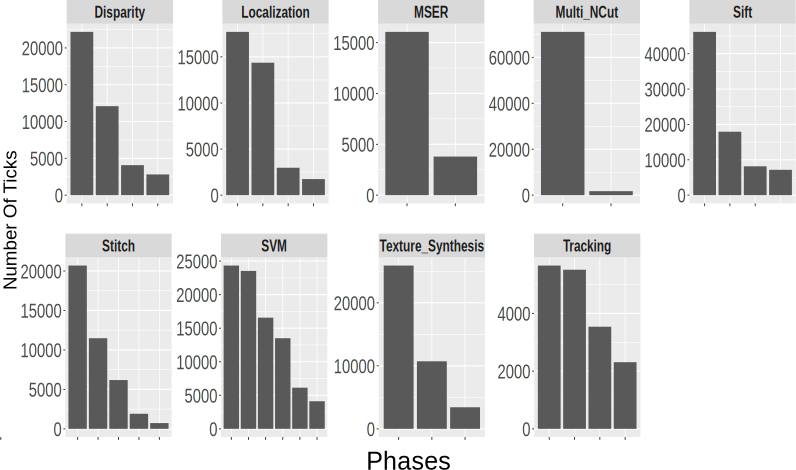
\includegraphics[width=1\textwidth]{cases-paper/graphics/Exploration/clusters3.pdf}
    \caption{Number of phases determined for each benchmark using kMeans clustering and their distribution.}
    \label{fig:clust}
		\vspace{5mm}
\end{figure}


\subsection{Phase Detection}
Figure~\ref{fig:sxt} presents the IPC performance through time for all the benchmarks when using a logical core (LC) composed of 16 cores.
The IPC is calculated for each time tick, which is set at interval of 640 blocks committed.
The IPC varies a lot for some of the benchmarks such as \bm{Disparity} or \bm{Localization} where dynamic fusion is expected to be especially good.
For other, such as \bm{Multi\_NCut}, the execution is dominated by a single long phase with constant IPC, which will clearly show no benefit from using dynamic fusion.

To better understand how dynamic core fusion improves performance, either by improving speedup or reducing energy, this section begins with a study of how each benchmark features different phases during their execution.
For every benchmark the IPC results of 16,8,4,2,1 fused cores are regrouped and kMeans clustering is applied to determine phases.
This process is only done for the purpose of exploring this set of benchmarks.
Intervals that exhibit similar IPC values when run on different core counts are classified in the same cluster.
In order to find the correct number of clusters the Sum of Square Errors (SSE) is plotted for a given cluster size from 1 to 15 and determine the optimal cluster to be in the elbow in the plot~\cite{everitCluster2001}.

Figure~\ref{fig:clust} shows us the optimal number of clusters for each benchmark and the frequency of each cluster.
The data can be corroborated with the information found in Figure~\ref{fig:sxt}.
For example, benchmarks \bm{MSER} and \bm{Multi\_NCut} feature two phases, with one dominating phase.
This means that it will be impossible to obtain any kind of performance improvements through dynamic reconfiguration.
For all the other benchmarks, they each have at least two dominant phases.
Since each phase is a cluster of similar IPC values, having two or more clusters will result in a higher chance of benefiting from dynamic core fusion.


\begin{figure}
    \centering
    \includegraphics[width=1\textwidth]{cases-paper/graphics/Exploration/stddev2.pdf}
    \caption{Comparing average, smallest and greatest IPC for each SD-VBS benchmark using logical-core size of 16.}
    \label{fig:stddev}
		\vspace{5mm}
\end{figure}

\begin{figure}[t]
    \centering
    \includegraphics[width=1\textwidth]{cases-paper/graphics/Exploration/SizeBuckets.pdf}
    \caption{Distribution of block sizes for each benchmark. The sizes were clustered in buckets equivalent to number of lanes occupied.}
    \label{fig:block_sizes}
	\vspace{5mm}
\end{figure}
\subsection{Static Core Fusion Exploration}

Figure~\ref{fig:stddev} shows how the average Instructions Per Cycle (IPC) changes as the size of a LC is increased, going in powers of 2 from 1 to 16 fused cores.
It can be seen that, for most benchmarks, fusing more cores provides an increase in IPC performance.
Benchmarks \bm{Disparity}, \bm{Localization}, \bm{Sift}, \bm{Stitch}, \bm{Texture Synthesis} and \bm{Tracking} all at least observe a speedup of 2x when using core fusion.

However increasing the size of a LC is not always beneficial as can be seen in benchmarks \bm{Localization}, \bm{MSER}, \bm{Multi\_NCut}, \bm{Stich}, and \bm{SVM}.
For benchmarks \bm{Localization} and \bm{Stitch} the performance increases when fusing up to 8 cores, where-as \bm{MSER} and \bm{Multi\_NCut} never benefit from core fusion. 
Referring back to Figures~\ref{fig:sxt} and~\ref{fig:clust}, \bm{MSER} and \bm{Multi\_NCut} feature one dominating long phase, both performing poorly.
Figure~\ref{fig:block_sizes} shows the distribution of block-sizes for each of the benchmarks.
As fine-grained sizes do not matter as much as overall number of lanes being occupied, the block sizes were clustered into groups which represent how ever many number of lanes will be occupied (one lane may execute a block of up to 32 instructions).

Figure~\ref{fig:block_sizes} helps explain why benchmarks \bm{MSER} and \bm{Multi\_NCut} do not perform any better with core-fusion.
For both cases, not only do they have a single detected phase, but both are predominantly formed of blocks that will occupy a single lane.
In fact, the most frequent block in \bm{MSER}, comprising 21\% the total executed blocks are comprised of only 8 instructions, whilst 31\% of \bm{Multi\_NCut}'s blocks are of 28 instructions.
Having such small blocks will always increase both the \textit{SynchronizationCost} and the branch-prediction requirements.
For \bm{MSER}, the fact that an important percentage of blocks are only 8 instructions long signifies that the overhead of fetching enough blocks for a large core-composition and the synchronization cost for committing them outweighs executing the blocks on a single core.
The reason there is no degredation of performance is due to the fact that when fusing a high amount of cores, if the overhead of fetching the blocks outweighs the time required to execute them, cores will simply not execute blocks.
For example, fusing 16 cores and executing \bm{MSER} may in fact result in a single core being used due to it executing blocks faster than it being able to dispatch the blocks to a next core.
Hence, in this case, \bm{MSER} would be wasting a lot of energy trying to use 16 cores in a composition, whilst effectively only executing on a single core. 
This explains the lack of scaling for these two benchmarks.

Figure~\ref{fig:stddev} also shows the standard deviation of the IPC for each given LC size represented by the grayed out areas.
For example, running the \bm{Disparity} benchmark on a LC of 16 cores, it can be observed that an average IPC of 8.3 with a standard deviation of 5.2.
The standard deviation for 16 cores shows that the performance can drop down to 2.5.
An IPC of 2.5 when using 16 cores is very inefficient as this represents 0.1 of an instruction per cycle for each core.
Using a LC of size 4 for the \bm{Disparity} benchmark we achieve an average of 4.1 with a standard deviation of 1.2.
Thus, if the logical-core could change size, there is a possibility that this could reduce the overall energy consumption of the system by switching from 16 to 4.

Overall, most benchmarks that benefit from large logical-cores will also be met with important standard deviations of IPC performance.
The high standard deviation is evidence of performance phases found in each application which are likely to benefit from dynamic adaptation.

\begin{figure}
     \centering
     \subfloat[][Disparity]{\includegraphics[width=0.5\textwidth]{cases-paper/graphics/Pareto/DispN3.pdf}\vspace*{-4mm}\label{subfig:disp}}
     \subfloat[][Localization]{\includegraphics[width=0.5\textwidth]{cases-paper/graphics/Pareto/LocN3.pdf}\vspace*{-4mm}\label{subfig:loc}}\
     \subfloat[][MSER]{\includegraphics[width=0.5\textwidth]{cases-paper/graphics/Pareto/MSERN3.pdf}\label{subfig:mser}}
     \subfloat[][Multi\_Ncut]{\includegraphics[width=0.5\textwidth]{cases-paper/graphics/Pareto/MultiN3.pdf}\label{subfig:mult}}\
     \subfloat[][Sift]{\includegraphics[width=0.5\textwidth]{cases-paper/graphics/Pareto/SiftN3.pdf}\label{subfig:sift}}
     \subfloat[][Stitch]{\includegraphics[width=0.5\textwidth]{cases-paper/graphics/Pareto/StitchN3.pdf}\label{subfig:stitch}}\
     \subfloat[][SVM]{\includegraphics[width=0.5\textwidth]{cases-paper/graphics/Pareto/SVMN3.pdf}\label{subfig:svm}}
     \subfloat[][Texture\_Synthesis]{\includegraphics[width=0.5\textwidth]{cases-paper/graphics/Pareto/TextN3.pdf}\label{subfig:text}}\\
     \subfloat[][Tracking]{\includegraphics[width=0.5\textwidth]{cases-paper/graphics/Pareto/TrackingN3.pdf}\label{subfig:track}}
     \caption{Time (x-axis) vs. Energy (y-axis) tradeoffs using Static and Dynamic Composition Schemes.}
     \label{fig:paretos}
\end{figure}
\newpage

\section{Dynamic Core Composition}\label{sec:dynamic}
This section discusses a dynamic core composition scheme that is created by generating traces of the ahead-of-time static compositions.
The section first describe how the traces are generated for the dynamic core composition schemes.
Before the analysis two types of static core composition are defined:

\begin{itemize}
	\item \textbf{Static Benchmark} (SB): A fixed fused-core which is optimal for a unique benchmark.
\vspace{-1.2em}
	\item \textbf{Static Suite} (SS): A fixed fused-core which represents the average best for the entire suite of benchmarks. This represents the baseline for the chapter.
\end{itemize}

The reason \textbf{Static Suite} is used as a baseline is due to the fact that it represents a configuration choice at design time.
It is the equivalent of hardware designers analysing the requirements of a processor based on the type of applications it will be executing.
This is better than using a single core as a baseline, as a single core will always represent the slowest execution time whilst also consuming the least amount of energy.
\textbf{Static Benchmark} on the other hand represents the ability to compose cores statically ahead of time; which is an extra step of flexibility compared to \textbf{Static Suite}.

The static core-composition scheme \textit{SS} is compared to the results obtained for the dynamic one for the SD-VBS benchmarks.
This is followed by a closer analysis of the dynamic core composition objective: optimising speed whilst reducing energy consumption.

\begin{figure}[t]
    \centering
	\includegraphics[width=1\textwidth]{cases-paper/graphics/exploration/trace-gathering.pdf}
    \caption{Overview of how traces are gathered to generate dynamic core composition traces.}
    \label{fig:tracegraph}
	\vspace{1em}
\end{figure}

\subsection{Creating Dynamic Core Composition Traces}

Dynamic core composition enables the ability to change the number of cores for each time tick (an interval of 640 committed blocks) during the execution of a program.
In order to explore the different performance and energy trade-offs that are possible to achieve with this technique, traces of execution for the application are collected.
Figure~\ref{fig:tracegraph} is a visual overview of how dynamic traces are collected.
First the application is executed on 1,2,4,8 and 16 composed cores and the performance is recorded for each time tick of 640 committed blocks.
Using these 5 traces, dynamic executions using any of the 5 different compositions can be constructed to generate dynamic traces.
For this chapter, the dynamic trace are generated based on maximising speed whilst minimising energy consumption.

To simplify the exploration process, time ticks that are attributed to the same phase are always given the same number of cores.
This is done to reduce the search space as on average there are 48,494 ticks which results in an average of $5^{48,494}$ different possible executions.
Since the maximum number of clusters found is 7 (for SVM), a maximum of $5^{7} = 78,125$ different dynamic execution traces can be built.
This is why creating dynamic core-composition out of traces is preferred to running all potential dynamic configurations via the simulator.
All applications run for a couple hundred million cycles, which often takes a couple of hours to execute.
As the amount of dynamic reconfigurations is high for some benchmarks, using traces to simulate dynamic reconfiguration is a very large time-save.

When the size of the core composition is switched, the performance of that composition from its respective trace file is used and an extra 100 cycle penalty is added for switching the size.
This 100 cycles is the overhead of reconfiguring the processor at runtime, the effect of the reconfiguration latency is discussed in further detail later on in this section.
The reconfiguration is a lightweight process as described in Chapter~\ref{chp:Background} section~\ref{sec:edge_arch} that involves informing the cores that they belong to a composition, which requires a write to a system register and potentially flushing pipelines if the cores are executing other threads.
As in this chapter, cores will never be executing other threads, flushing is not necessary, thus the l00 cycles to inform cores is an appropriate penalty and has been used in previous studies on DMPs~\cite{pricopi2012bahurupi}.
With all these different dynamic core composition traces, the optimal schemes for efficiently maximising speed can be found.

\begin{figure}[t]
    \centering
	\includegraphics[width=1\textwidth]{cases-paper/graphics/pareto/pareto_best.pdf}
\vspace{-1em}
    \caption{Time (x-axis) vs. Energy (y-axis) trade-offs using Static and Dynamic Composition Schemes.}
    \label{fig:paretos}
	\vspace{1em}
\end{figure}

%\begin{figure}[t]
%     \centering	%
%	 \vspace{-1em}
%     \subfloat[][Disparity]{\includegraphics[width=0.33\textwidth]{cases-paper/graphics/Pareto/DispN3.pdf}\vspace*{-4mm}\label{subfig:disp}}
%     \subfloat[][Localization]{\includegraphics[width=0.33\textwidth]{cases-paper/graphics/Pareto/LocN3.pdf}\vspace*{-4mm}\label{subfig:loc}}
%     \subfloat[][MSER]{\includegraphics[width=0.33\textwidth]{cases-paper/graphics/Pareto/MSERN3.pdf}\label{subfig:mser}}\
%	 	 	 \vspace{-0.5em}
%
%     \subfloat[][Multi\_Ncut]{\includegraphics[width=0.33\textwidth]{cases-paper/graphics/Pareto/MultiN3.pdf}\label{subfig:mult}}
%     \subfloat[][Sift]{\includegraphics[width=0.33\textwidth]{cases-paper/graphics/Pareto/SiftN3.pdf}\label{subfig:sift}}
%     \subfloat[][Stitch]{\includegraphics[width=0.33\textwidth]{cases-paper/graphics/Pareto/StitchN3.pdf}\label{subfig:stitch}}\
%	 	 	 \vspace{-0.5em}
%
%     \subfloat[][SVM]{\includegraphics[width=0.33\textwidth]{cases-paper/graphics/Pareto/SVMN3.pdf}\label{subfig:svm}}
%     \subfloat[][Texture\_Synthesis]{\includegraphics[width=0.33\textwidth]{cases-paper/graphics/Pareto/TextN3.pdf}\label{subfig:text}}
%     \subfloat[][Tracking]{\includegraphics[width=0.33\textwidth]{cases-paper/graphics/Pareto/TrackingN3.pdf}\label{subfig:track}}
%     \caption{Time (x-axis) vs. Energy (y-axis) tradeoffs using Static and Dynamic Composition Schemes.}
%     \label{fig:paretos}
%	 	 	 	 \vspace{1em}
%\end{figure}

\subsection{Dynamic Core Composition}
Figure~\ref{fig:paretos} shows the trade off between time (cycles) and energy using either a static ahead of time or dynamic (re)-configuration.
The dotted line represents the static core composition scheme for the benchmark whilst the solid line represents the Pareto Front of all the dynamic core composition traces.
The vertical line represents the amount of energy that can be saved from using a dynamic core composition scheme that matches the same speed as the best static scheme.
The Pareto Front is constructed by assigning different core composition sizes to a phase and recording the execution time in cycles and energy consumption.
For a given cycle count, the reconfiguration scheme that leads to the smallest energy consumption is chosen to be a point in the Pareto Front.

Figure~\ref{fig:paretos} demonstrates how static core-composition fails to maintain good energy efficiency as speed is improved.
For example, \bm{Disparity} is fastest on 16 fused cores, but has an 1.63x increase in energy consumption for a 1.22x improvement in speed.
This is due to the fact that larger core compositions do not result in linear speedups, and thus consume more energy than a smaller core composition.
When using the dynamic scheme, it is clear that energy consumption increases at a slower rate when increasing speed.
In this case the number of cores is adapted to the current phase, using just enough cores to maintain high performance without wasting energy.

Figure~\ref{fig:paretos} also shows how very few applications get faster execution times with dynamic core composition.
The main program that does perform better execution wise with dynamic core composition is \bm{Localization}.
In the case of \bm{Localization}, the fastest execution time using static core-composition comes from a logical core of size 8.
However, there are certain phases that perform better with 16 cores, and thus, dynamic core composition in this situation can lead to faster execution times.
Overall, for these benchmarks, most have their fastest execution times with a static core-composition.
Dynamic reconfiguration is therefore mainly used to limit the energy consumption.

\subsection{Optimising for Speed} \label{sec:dyn:speed}

In this section the dynamic scheme is defined to be one that matches the same speed performance as the fastest static core composition for the benchmark: \textbf{DSpeed}.
This is equivalent to the vertical line found in Figure~\ref{fig:paretos}.
This scheme is used to demonstrate how dynamic reconfiguration can achieve the same speed as the static configuration whilst reducing energy consumption.

Figure~\ref{fig:speedres} shows the speedup of \textbf{DSpeed} and Static Best (SB) and the respective energy consumption.
The results are normalised against the performance of Static Suite (SS), which is 8 cores fused.
The SS core count is obtained by averaging the number of cores that leads to the fastest execution time for each benchmark.
The execution times for \textbf{DSpeed} and SB are the same as the dynamic scheme designed to match the static best's execution time.
As can be seen some benchmark perform better when using benchmark specific core compositions rather than SS.
Both \bm{Disparity} and \bm{Sift} obtain a 1.25x speedup when using the SB scheme whilst \bm{Tracking} benefits from a 1.10x speedup.
This reconfirms the concept that even static core-composition is a feature that leads to performance improvements over design time configurations.

\begin{figure}[t]
    \centering
	\includegraphics[width=1\textwidth]{cases-paper/graphics/results/speed_bars3.pdf}
\vspace{-1em}
    \caption{Maximising speed for all the SD-VBS benchmarks. For Speedup, higher means better, for Energy, lower is better.}
    \label{fig:speedres}
	\vspace{1em}
\end{figure}

When looking at the Energy graph of Figure~\ref{fig:speedres}, it is clear where the SS scheme fails.
Benchmarks \bm{MSER} and \bm{Multi\_NCut} feature very little improvement when using core composition, if any, therefore SS will perform very poorly when it comes to energy consumption for the benchmarks.
In the case of those benchmarks, the energy consumption is over 2x less on SB than it is on SS.
In this situation, SS is analogous to designing a large physical core meant to extract a lot of IPC for single-threaded performance and executing low IPC benchmarks on it.
This core will end up consuming too much energy and lead to low performance increases.
SB already shows the advantages of designing smaller, simpler physical cores which can be composed ahead of time.
For applications such as \bm{MSER} or \bm{Multi\_NCut}, a single low energy core suffices whereas \bm{Disparity} and \bm{Tracking} benefit from large compositions for better speedup.

However, SB is still not an optimal solution. 
For the benchmarks \bm{Disparity}, \bm{Sift}, \bm{Texture\_Synthesis} the energy consumption is much higher.
This is due to the fact that these benchmarks perform best on a 16-core system, however as seen in Figure~\ref{fig:stddev}, the variation in performance always increases when fusing this many cores.
In this situation, whilst 16 cores does result in the fastest execution times, the energy consumption is higher than SS.
This shows the limitations of static configuration overall, whether it be at design time or ahead of time: the lack of flexibility means that compromises have to be made.
In the case of aiming for the fastest execution times energy consumption may increase.

%More here
The dynamic reconfiguration \textbf{DSpeed} scheme always performs better than the SB scheme in terms of energy consumption and can even match the SS scheme on energy consumption whilst improving speed such as in the \bm{Sift} benchmark.
For the \bm{Localization} benchmark, the \textbf{DSpeed} matches the performance of both the SB and SS whilst reducing energy consumption by 65\%.
By using \textbf{DSpeed}, the energy consumption can be reduced by 42\% compared to both SB and SS without impacting performance.
This illustrates the greatest advantage of using a DMP since the number of composed core can be adapted continuously depending on the amount of ILP available.

\subsection{Reconfiguration Latency} \label{sec:reconfoverhead}

\begin{figure}[t]
	\begin{minipage}{.5\textwidth}
	\includegraphics[width=.9\linewidth]{cases-paper/graphics/Exploration/condensed_clust.pdf}
    \caption{Average number of cycles without switching.}
    \label{fig:avlen}
	\end{minipage}%
	\begin{minipage}{.5\textwidth}
	\hfill
	\includegraphics[width=.9\linewidth]{cases-paper/graphics/Exploration/latency_2.pdf}
    \caption{Energy savings and number of switches as a function of the switching latency in cycles.}
    \label{fig:enlatency}
\end{minipage}
\vspace{5mm}
\end{figure}

%Check if th
Up until now, the chapter has assumed a reconfiguration latency of 100 cycles whenever dynamic reconfiguration occurs as explained in Chapter~\ref{chp:setup}.
This section studies the impact of a larger reconfiguration overhead on energy savings.
First, figure~\ref{fig:avlen} shows the average phase length for each benchmark when maximising energy savings while maintaining performance (\textbf{DSpeed}).
As can be seen, the majority of the benchmarks run for long period of several tens of thousands of cycles before any switching occurs on average.
Therefore, even if the reconfiguration latency is increased to a larger value (\eg 1,000 cycles), its impact might be minimal.
For these applications, the phase length is also tied to the size of the input, the phases may increase when working on inputs such as high definition images.

Furthermore, there is always the option to reconfigure less often, in the case where a change in configuration only brings marginal reduction in energy.
In such case it might be more beneficial to keep running on the slightly less optimal configuration than paying a cost for reconfiguration.
Figure~\ref{fig:enlatency} illustrates this perfectly, showing how energy behaves as a function of the reconfiguration overhead (averaged across benchmarks).
For each latency value, the best trace of reconfiguration is determined to keep performance equal to the best static configuration while minimising energy (\textbf{DSpeed}).
The left y-axis expresses the energy savings relative to the static scheme, while the right y-axis shows the total number of switches.
The energy savings remains high up to a latency of 1,000 cycles, with a noticeable decrease in the number of switches.
For latency values over 1,000 cycles, the energy savings drop considerably, with very little switching occurring.
This data shows that even if the reconfiguration overhead is 1,000 cycles, average energy savings of 38\% are possible compared to 42\% when the overhead is 100 cycles.

\paragraph*{Summary}

Overall, dynamic core composition will always lead to higher speedup with lower energy consumption compared to a fixed configuration.
This is due to the presence of phases in applications that the dynamic scheme can exploit to reduce wasting energy in low ILP phases.
This section has shown that maximising speed can be highly energy inefficient when using a static composition and that a dynamic scheme can help reduce energy consumption by 42\% on average.




\section{Linear Regression Model}\label{sec:model}
The previous section showed that dynamically reconfiguring the processor can help reduce energy consumption whilst still achieving the same execution time as the fastest ahead of time configuration.
In order to benefit fully from dynamic core-composition two solutions are possible; either the programmer must go through the code and manually determine when to change the composition or an automatic scheme can be deployed.
This section now presents a learning scheme that is used to exploit the large energy savings available.
The main idea is to monitor at runtime some performance counters and make a decision at a regular interval on how to reconfigure the cores.
For this purpose, a model is trained offline using the data collected and presented earlier in the chapter.
Once trained, the model predicts the optimal number of cores based on the performance counters from the previous time interval and reconfiguration occurs if it is different from the current number of cores.

\begin{figure}[t]
    \centering
	\includegraphics[width=1\textwidth]{cases-paper/graphics/other/model3.pdf}
	\vspace{-2em}
    \caption{Linear Model.}
    \label{fig:linmod}
\end{figure}
\subsection{Model}

As the decisions are made at runtime, a lightweight model that is able to predict the correct configuration that can be integrated in hardware is necessary.
Linear regression, which makes predictions using a weighted sum of the input feature, has been demonstrated to be useful for predicting processor performance~\cite{Joseph2006LinReg}.
It is chosen as it has been as it can easily be implemented in hardware~\cite{lee2006linreg,Lukefahr2012Composite} and has a low overhead when computing the sum.
The model is trained offline using the traces gathered from the prior analysis for the \textbf{DSpeed} scenario which maximises energy savings while maintaining performance.

Figure~\ref{fig:linmod} is a shows how the linear model is trained.
The dataset consists of a set of four input features (average block size, and percentage of integer, floating point and load operations) and the optimal number of cores for each time tick for each program.
These features are chosen as they are easy to extract from the hardware.
The reason stores are not in the feature vector is due to the fact that a block is comprised only of integer, floating point, load and store operations.
Therefore, when building the model, a correlation analysis determined that stores correlate with other features and selects to remove it as a variable.
 % a single data point is created per phase, averaging the features of all the ticks in a phase, resulting in a total of 34 pairs of optimal core number and features.

To speedup the learning process, for each benchmark the features of all the ticks in a phase were averaged out to create a single data point, which is comprised of an IPC value, and the features described in Figure~\ref{fig:linmod}.
This averaging out leads to 34 data points for all the benchmarks.
The training consists of finding the weights that minimise the error when predicting the optimal number of cores to use across all time ticks and benchmarks.
Since only core configurations which use a power of two number of cores are considered, the linear model is built to predict the logarithm (base 2) of the number of cores.
The prediction is rounded up to the nearest integer in the interval $[0,4]$.
The following equation represents the trained linear model which can be used to make prediction:
\vspace{-1em}
\begin{align*}
  log_2(\textbf{\#cores}) = & -7.7\ +\ 0.028 \cdot \textbf{avgBlkSze}\ +\ 0.075 \cdot \textbf{\%int\_ops}\ +\\
 &0.069 \cdot \textbf{\%fp\_ops}\ +\ 0.21 \cdot \textbf{\%ld\_ops}
\end{align*}

It is important to note that this model was not used during the validation, as cross-validation (see Chapter~\ref{chp:Background}) was used to evaluate it.
Instead, this represents a model where the data from all programs is used.
For instance, if at runtime an average block size of 6 instructions, and 77\%, 1\% and 18\% of integer, floating point and load operations, respectively, then the predicted value will be 2.092.
Rounded up to the nearest integer value, 2, the optimal number of cores predicted will, therefore, be 4.

As can be seen, the largest weight is on the percentage of loads operations.
This is due to different reasons, mainly execution time and the fact that Load-Store Queues are fused.
When it comes to execution time, loads may take from 3 to 128 cycles depending on whether or not it is a cache miss or hit.
Whether it is a cache hit or miss, a block that takes longer to execute will often minimise the \textit{SynchronisationCost} penalty.
A block composed mainly of integer or floating point operations will often result in shorter execution rates; thus may execute faster, making it harder for large logical cores to improve performance.

More discussion on how the time it takes to execute a block influences the performance of core compositions is discussed in Chapter~\ref{chp3}.
The other reason loads have the largest weight is due to the fact that loads can be fired independently to the Load-Store Queue.
Unlike stores that depend on previous memory instructions blocks being committed, loads can be fired with less overhead.
As data can be speculatively fetched, load instructions can receive data from other cores before the data is stored, speeding up executions.
By increasing the core count on load heavy blocks this will improve performance more reliably due to cores being able to issue loads in parallel.

\begin{figure}[t]
    \centering
	\includegraphics[width=1\textwidth]{cases-paper/graphics/results/lr_speed3.pdf}
    \caption{Performance results for maximising speed for the SD-VBS benchmarks using the linear regressor (LR) model. The results are normalised against the Static Suite core composition.}% For Speedup, higher means better, for energy lower is better.}
    \label{fig:speedlr}
	\vspace{1em}
\end{figure}

%explain why MSER here is bad. Most likely because it over-estimates because some features in the vector don't describe the performance in the application.
%This is most likely due to the branch prediction/.
\subsection{Results}

To evaluate the performance of the model leave-one-out cross-validation  is used; it is a standard machine-learning methodology which tests the model using not seen during training.
For instance, if the model is tested for one program, let say \textit{Disparity}, the model is then trained using the dataset from all the other programs combined.
Then the resulting trained linear model is used to predict the optimal core number for each time tick of the disparity program and report the performance achieved.

Figure~\ref{fig:speedlr} shows the performance in terms of speed and energy that is achieved using the linear model normalised by a fixed static configuration.
The fixed configuration maximised performance across all the benchmarks using 8 cores and is the same as in the previous results presented in figure~\ref{fig:speedres}.
On average, the linear regressor model is able to consume 37\% less energy compared to the 8 cores fixed configuration and is able to exactly match its speed.
The main outlier is \bm{MSER} where the linear regressor consumes over 2x more energy than \textbf{DSpeed}.
This is due to the fact that \bm{MSER} is a benchmark where the branch prediction is poor as previously mentioned in Table~\ref{tab:sd-vbsbpred}.
Indeed, \bm{MSER} has an average branch prediction of 85\% compared to the average of 95\%.S
As \bm{MSER} tends to have very small blocks, the branch prediction makes it very difficult to ever efficiently use even a core composition of size 2.
This benchmark is therefore an outlier compared to the rest of the set, as it is the branch prediction causing incorrect predictions from the linear regression.

The performance is also compared with the best possible choice of dynamic reconfiguration, \textbf{DSpeed} which acts as an Oracle.
As can be seen, the linear model is able to exploit similar energy savings to the \textbf{Dspeed} scheme in most cases.
On average it reduces energy by 37\%, which is within 5\% of the 42\% achievable by the \textbf{Dspeed} scheme.
These results show that it is possible to implement a simple realistic lightweight scheme which offers large energy savings.


%\section{Related Work}\label{sec:related}
%
\paragraph{Reconfigurable Processors}

ElasticCore~\cite{tavanaElastic} proposes a morphable core that uses dynamic voltage and frequency scaling (DVFS) and microarchitectural modifications such as instruction bandwidth and capacity.
They propose a linear regressor model to determine reconfiguration, which uses more runtime information than ours, such as branch prediction and cache misses.
Overall Tavana et al's architecture is 30\% more energy efficient than a big.LITTLE architecture.

In~\cite{dubach13dynamic} they also propose a similar core architecture that modifies microarchitectural features.
They provide extensive analysis of SPEC 2000 benchmarks and demonstrate that machine learning and dynamic adaptation can double the energy/performance efficiency compared to a static configuration.

MorphCore~\cite{khubaibMorphCore2012} focuses on reconfiguring a core for thread level parallelism.
It switches between out-of-order (OoO) when running single threaded applications and an in-order core optimised for simultaneous multi threading (SMT) workloads.
This provides an opposite solution to our DMP: providing a large core made for ILP that can be modified to better fit TLP workloads.
MorphCore outperform a 2-Way SMT OoO core by 10\% whilst being 22\% more efficient.

All these projects focus on uni-core modifications, and traditional CISC/RISC like architecture which differs from our work.

\vspace{-0.5em}
\paragraph{Dynamic Multicore Processors}
Previous work on Dynamic Multicore Processors includes CoreFusion~\cite{ipek2007CoreFusion} and Bahurupi~\cite{pricopi2012bahurupi,pricopiSchedCoreComp2014}.
These architectures use a standard ISA and either fetch fixed sized instruction windows~\cite{ipek2007CoreFusion} or entire basic blocks~\cite{pricopi2012bahurupi}.
Other DMPs such as TFlex~\cite{kim2007tflex} and E2~\cite{e2} use an hybrid-dataflow EDGE ISA~\cite{burger04edge}. 
In TFlex, instructions from a block are executed on different fused cores.
In E2, a block is mapped to a fused core and all instructions from that block execute locally.

\vspace{-0.5em}
\paragraph{Dynamic Core Fusion}
In the work of Pricopi {\it et al.~}~\cite{pricopiSchedCoreComp2014}, they show how dynamic reconfiguration is beneficial when it comes to scheduling tasks.
However, they do not discuss any method of automatically deciding the optimal configuration beyond a 4 core fusion.
Instead they use speedup functions determined from profile executions of applications to determine how to schedule tasks.
They do not discuss what software characteristics help determine when to reconfigure the cores, or how to optimise software.

Work on using machine learning to automatically choose a composition was achieved in~\cite{micolet2016dmpstream}.
This work does not involve changing the core fusion dynamically during the execution of the benchmark.
The machine learning model focuses on using high-level information from StreamIt's~\cite{thiesStreamit2010} language constructs.

\vspace{-0.5em}
\paragraph{Voltage Scaling}
Voltage scaling is another method of reducing energy consumption~\cite{paganiEECHM2017}, however this approach is orthogonal to DMPs~\cite{sibi}.
Whilst both methods adapt to programs phases, DMPs can also be used to speed up the execution of programs.


\section{Conclusion}\label{sec:conc}
This chapter tackled the problem of dynamic reconfiguration of a Dynamic Multicore Processor at runtime.
Due to the fact that adding cores in a core-composition does not result in linear improvements, obtaining the fastest performance comes at the cost of energy.
Therefore, static core compositions are not an efficient method to speed up programs with phases.
Runtime dynamic reconfiguration of DMPs is therefore necessary to ensure that core compositions are used appropriately.

To better understand how core-composition is sensitive to branch prediction and block size, a limit study is conducted.
It shows that larger core-compositions favour large blocks as this reduces the strain on the branch predictor and also reduces the communication cost between cores.
To improve the size of blocks and block level parallelism, a set of compiler optisations such as loop inversion, loop unrolling and predication are discussed.

These optimistions are then applied on a set of vision benchmarks, and the performance of static core-compositions help show that these programs have phases of IPC patterns.
Using this information, two dynamic runtime reconfiguration schemes are created:  \textbf{DSpeed} that matches the speed of the fastest static core fusion and \textbf{DEff} that maximizes efficiency.
The chapter shows that \textbf{DSpeed} saves on average 42\% energy compared to the optimal static logical core whilst \textbf{DEff} can improve performance by up to 1.30x and reduce energy consumption by 1.20x on some benchmarks.

Finally a linear regression model is proposed to decide the number of cores to fuse at runtime for \textbf{DSpeed}.
This  model leads to a 37\% reduction in energy whilst maintaining the same level of performance as the optimal static scheme.

Overall, the contributions of this chapter are:

\begin{itemize}
\item Analysis of the limits of core fusion using an analytical model.
\vspace{-1em}
\item A study of the loop optimizations required to ensure efficient use of core fusion.
\vspace{-2.5em}
\item An in-depth comparison of static and dynamic core fusion schemes on the San Diego Vision Benchmark Suite.
\vspace{-1em}
\item A demonstration that core fusion has the potential to offer a large reduction in energy savings.
\vspace{-1em}
\item A demonstration that a simple linear-regression based model can predict the number of cores to fuse for different program phases.
\end{itemize}

%In this paper we have shown that whilst static core fusion already demonstrates promising results, it becomes harder to be efficient when increasing the size of logical cores.
%We explained theoretical limitations of static core fusion; without high branch prediction and large blocks, it under-performs.
%This was followed by a study of a suite of benchmarks, showing how performance varies greatly depending on the size of logical cores. 

%We then created two dynamic schemes: \textbf{DSpeed} that matches the speed of the fastest static core fusion and \textbf{DEff} that maximizes efficiency.
%Using these schemes we saw that \textbf{DSpeed} saves on average 42\% energy compared to the optimal static logical core for a given benchmark.
%We also showed that \textbf{DEff} can improve performance by up to 1.30x and reduce energy consumption by 1.20x on some benchmarks.
%Finally, we developed a simple linear regression model to decide on the number of cores to fuse at runtime to optimize for performance, leading to a 37\% reduction in energy while maintaining the same level of performance as a static scheme.


